\documentclass[11pt]{article}
\usepackage[margin=1in]{geometry}
\usepackage[dvipsnames]{xcolor}
\usepackage{graphicx,booktabs,amsmath,hyperref,caption,placeins}
\usepackage[T1]{fontenc}
\captionsetup{font=small,labelfont=bf}
\hypersetup{colorlinks=true,linkcolor=blue!50!black,urlcolor=blue!50!black}
\graphicspath{{../fpe_report/figs_pool/}{../fpe_report/figs_vote_perfeature/}}

\title{A pooled ensemble of independently trained latent models\\ for CM1 squall-line forecasts}
\author{Dalton Jones \and Claude}
\date{23 November 2026}

\begin{document}
\maketitle

\begin{abstract}
We describe a learned forecast system for two-dimensional CM1 squall lines. It has three parts:
\begin{itemize}
\item a stochastic latent model: a convolutional column autoencoder and a mixer propagator with noise channels, trained with a fair-CRPS rollout loss on 573 simulated storms;
\item a pool of several copies of this model, trained independently with different random seeds, whose members are combined into one ensemble;
\item a vote that turns the ensemble into yes/no forecasts of storm features such as updrafts, downdrafts, the cold pool and the mesolow.
\end{itemize}
On 22 storms never used in training, a pool of four models beats a single model with the same number of members. Fair CRPS is 3.3--5.2\% lower at every lead from 5 to 90 minutes, the ensemble-mean error is 1.4--3.8\% lower, and the vote's critical success index (CSI) is higher for every feature. The pool's spread is also calibrated (spread/error $\approx 1.0$) without any tuning. We close with what the system implies for ensemble data assimilation.
\end{abstract}

\section{The model}

\paragraph{Data.} The training data are 2D ($x$--$z$) CM1 squall lines with the following setup:
\begin{itemize}
\item a 400\,km by 20\,km domain with 250\,m grid spacing and 62 stretched levels;
\item Morrison two-moment microphysics, open lateral boundaries, and a grid moving at 12.5\,m\,s$^{-1}$;
\item 1-minute output for 6\,h.
\end{itemize}
A model state is the column at every grid cell: $u'$, $w$, $\theta'$, $q_v'$, $p'$, and liquid and ice condensate (as $\sqrt{q}$) on 62 levels, i.e.\ 434 channels per column. There are 601 storms. They share one squall-line sounding and differ in boundary-layer moisture, near-surface temperature and low-level shear. We train on 573 of them, keep 6 for validation (all tuning, including the vote cutoffs) and 22 for testing. No test storm is used in any choice.

\paragraph{One model.} Each model has two networks.
\begin{itemize}
\item \emph{Autoencoder} (5.0\,M parameters): a convolutional encoder maps 8 neighbouring columns (2\,km) to one site with 32 latent channels. It has two local mixing layers (hidden width 416), and the decoder mirrors it. The latent state is a field on a 1D lattice of 2\,km sites, not a single vector, so the model works on any domain length.
\item \emph{Propagator} (11.9\,M parameters): a mixer network (GELU, LayerNorm, width 512, 3 layers, reach of one site per layer). It advances the latent field by one minute as a residual update. It is stochastic: 4 Gaussian noise channels are fed in at every step, so repeated rollouts from one initial state give different ensemble members. The outermost 3 sites (6\,km) on each side form a halo that is set from outside the domain.
\end{itemize}

\paragraph{Training.} Training has three stages, all on one H200 GPU, and takes about 4.5\,h per model.
\begin{enumerate}
\item[A.] \emph{Autoencoder}, 60\,k steps on 64\,km windows. The loss is reconstruction plus a one-step prediction term, in which a small propagator must predict the next minute from the latent. Nested dropout on the latent channels and weak variance and log-determinant terms prevent channel collapse.
\item[B.] \emph{Propagator} on the frozen latent, 40\,k steps on 96\,km windows. Rollouts are up to 45 minutes long, with a length that ramps up during training, and are scored by the fair CRPS of 4 sampled rollouts against the encoded truth.
\item[C.] \emph{Joint fine-tuning}, 30\,k steps. Rollouts to 45 minutes are decoded, and the fair CRPS is computed in physical space against the true fields, with extra weight on surface $\theta'$. The autoencoder is not frozen, so the latent space adapts to be forecastable.
\end{enumerate}
The fair CRPS rewards a set of members that is both accurate and spread like the truth, so each member keeps sharp, realistic small-scale structure rather than a smoothed average.

\paragraph{The pool.} A pool is $n$ copies of the model trained with the same recipe and data but different random seeds (initialization, sampled windows, noise). Each copy works as a separate model. It encodes the initial state with its own encoder, rolls out its own members, and decodes them with its own decoder. The members are combined in physical space. The standard pool is 4 models $\times$ 8 members.

\paragraph{The vote.} To forecast \emph{where} a feature will be, every member is turned into a 0/1 mask with a fixed physical threshold. The 12 features are:
\begin{itemize}
\item updraft $w>2$\,m\,s$^{-1}$ and downdraft $w<-1.5$\,m\,s$^{-1}$;
\item $u'>10$ and $u'<-10$\,m\,s$^{-1}$;
\item cold pool $\theta'<-2$\,K and warm core $\theta'>5$\,K;
\item moist $q_v'>1$\,g\,kg$^{-1}$ and dry $q_v'<-3$\,g\,kg$^{-1}$;
\item mesohigh $p'>3$\,hPa and mesolow $p'<-1$\,hPa;
\item liquid $>0.5$\,g\,kg$^{-1}$ and ice $>1$\,g\,kg$^{-1}$.
\end{itemize}
A grid point is forecast to have the feature if at least $K$ of 8 members have it. $K$ is chosen per feature and lead to maximize CSI on the validation storms. It is 3 or 4 for most features and 2--3 for downdrafts. For larger ensembles the cutoff is kept as a fraction, $K_S=\lceil K_8 S/8\rceil$ for $S$ members. Figure~\ref{fig:howvote} shows the vote on one storm.

\begin{figure}[h]
\centering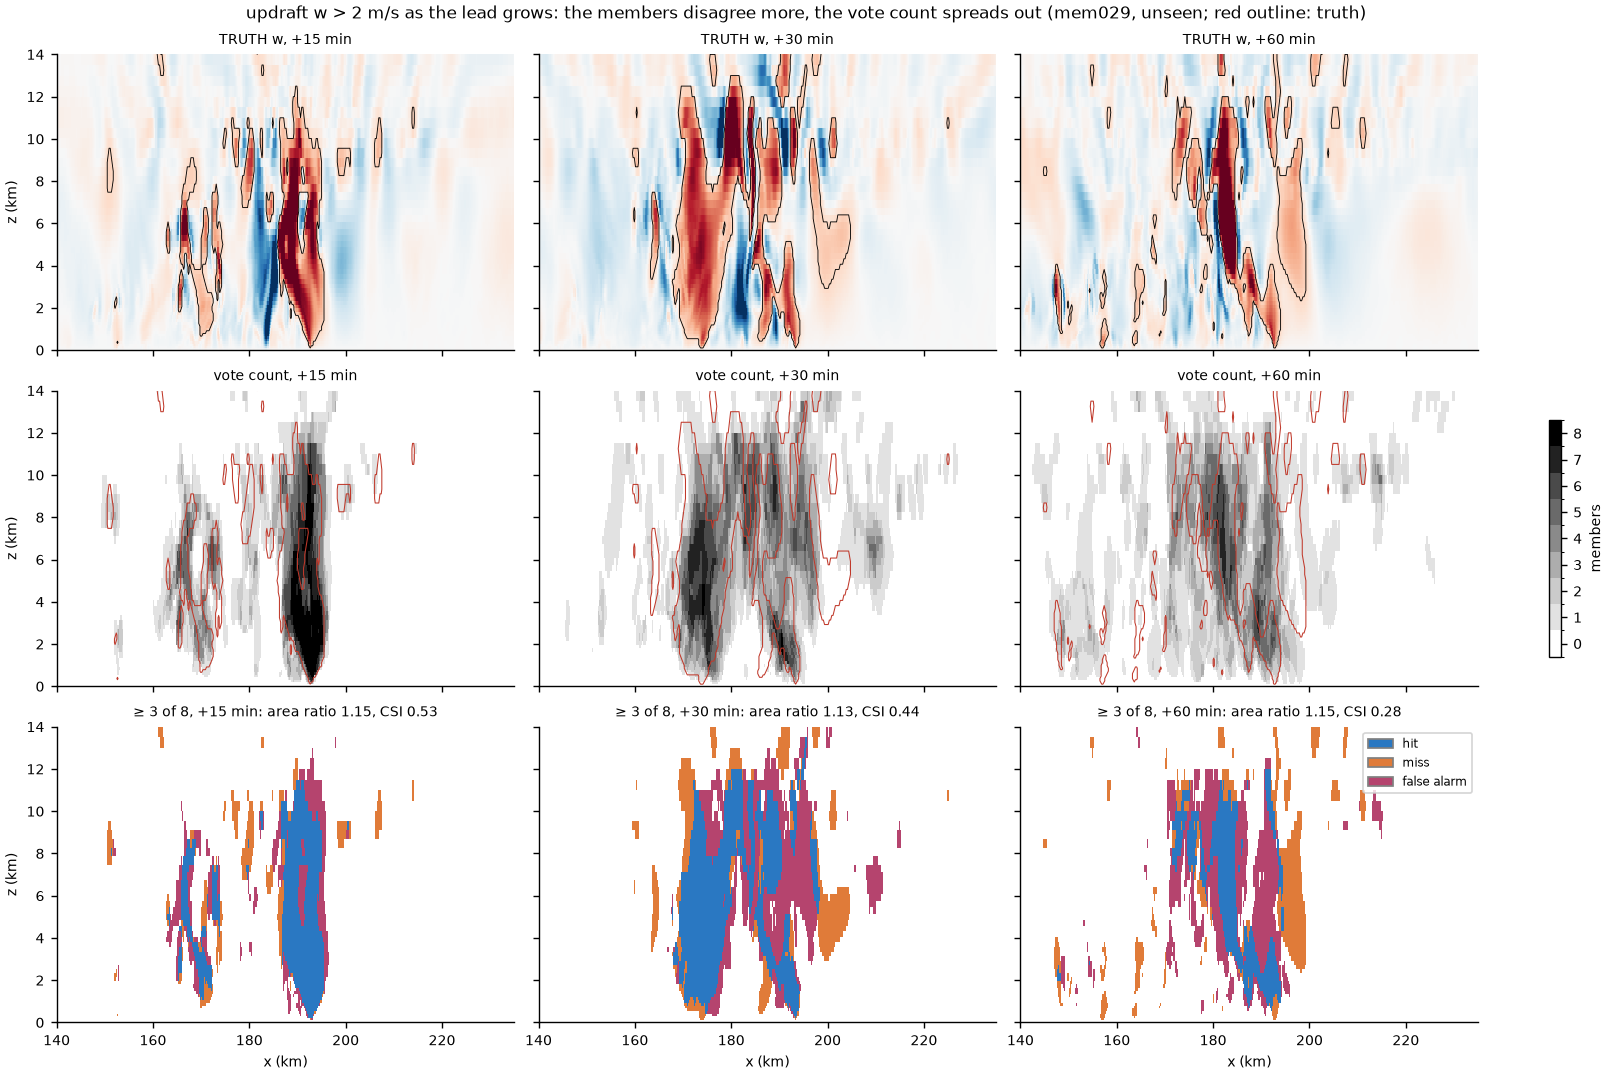
\includegraphics[width=\textwidth]{fig_vote_leads_wp_mem029.png}
\caption{The vote for updrafts on an unseen storm at +15, +30 and +60\,min (one model, 8 members). Top: truth. Middle: how many members have an updraft at each point (red: true outline). Bottom: the voted forecast as hits, misses and false alarms.}
\label{fig:howvote}
\end{figure}

\FloatBarrier
\section{How well does it forecast?}

\paragraph{Setup.} Forecasts start from the encoded true state at 1, 2 and 3\,h into each of the 22 test storms (66 cases) and run to 90 minutes. The halo is set from the true state; holding it at its starting value instead raises CRPS at 60\,min by about 4\%. The scores are:
\begin{itemize}
\item the fair CRPS per variable, in normalized units;
\item the RMSE of the ensemble mean;
\item the spread/error ratio, where 1 means calibrated;
\item for the vote, CSI and frequency bias (forecast area / true area).
\end{itemize}

\paragraph{Pool against single models.} We compare ensembles with the same number of members (24): each of four seeds alone with 24 of its own members, and pools of three and four models (Fig.~\ref{fig:skill}, Table~\ref{tab:pool}).
\begin{itemize}
\item \emph{Probabilistic skill.} Pooling lowers CRPS by 3.3--5.2\% at every lead. The four seeds alone differ from each other by at most 0.8\%, so the gain is more than four times the seed-to-seed spread. It passes the decision rule we fixed before the run: more than $2\times$ the seed spread and at least 2\%.
\item \emph{Calibration.} The ensemble-mean RMSE improves by 1.4--3.8\%, most at short leads. A single model is slightly under-dispersive (spread/error 0.91--1.01). The pool's spread/error is 0.99--1.03. Part of the forecast error comes from the trained model itself. Members of one model all share that model's errors, whereas independently trained models make different errors, so their spread covers this part.
\item \emph{How many models.} Three models give about 90\% of the CRPS gain of four.
\item \emph{By variable.} The gain holds for every variable and lead (Fig.~\ref{fig:pervar}). It is largest for $u$ and $q_v$ (5--6\% in CRPS) and smallest for $w$ and liquid water beyond 15\,min (1--2.4\%).
\end{itemize}

\begin{table}[h]
\centering\small
\begin{tabular}{lcccc}
\toprule
lead & CRPS, single model (4 seeds) & CRPS, pool of 4 & change vs mean single & spread/error, single $\to$ pool \\
\midrule
15\,min & 0.0747--0.0758 & 0.0720 & $-4.2\%$ & 0.95 $\to$ 1.01 \\
30\,min & 0.0951--0.0955 & 0.0920 & $-3.5\%$ & 0.96 $\to$ 1.00 \\
60\,min & 0.1174--0.1181 & 0.1139 & $-3.3\%$ & 0.99 $\to$ 1.02 \\
90\,min & 0.1336--0.1347 & 0.1293 & $-3.5\%$ & 0.97 $\to$ 1.01 \\
\bottomrule
\end{tabular}
\caption{Fair CRPS (mean over the 7 variables, normalized units) of 24-member ensembles: single models against the pool of four (6 members per model). 66 cases.}
\label{tab:pool}
\end{table}

\begin{figure}[h]
\centering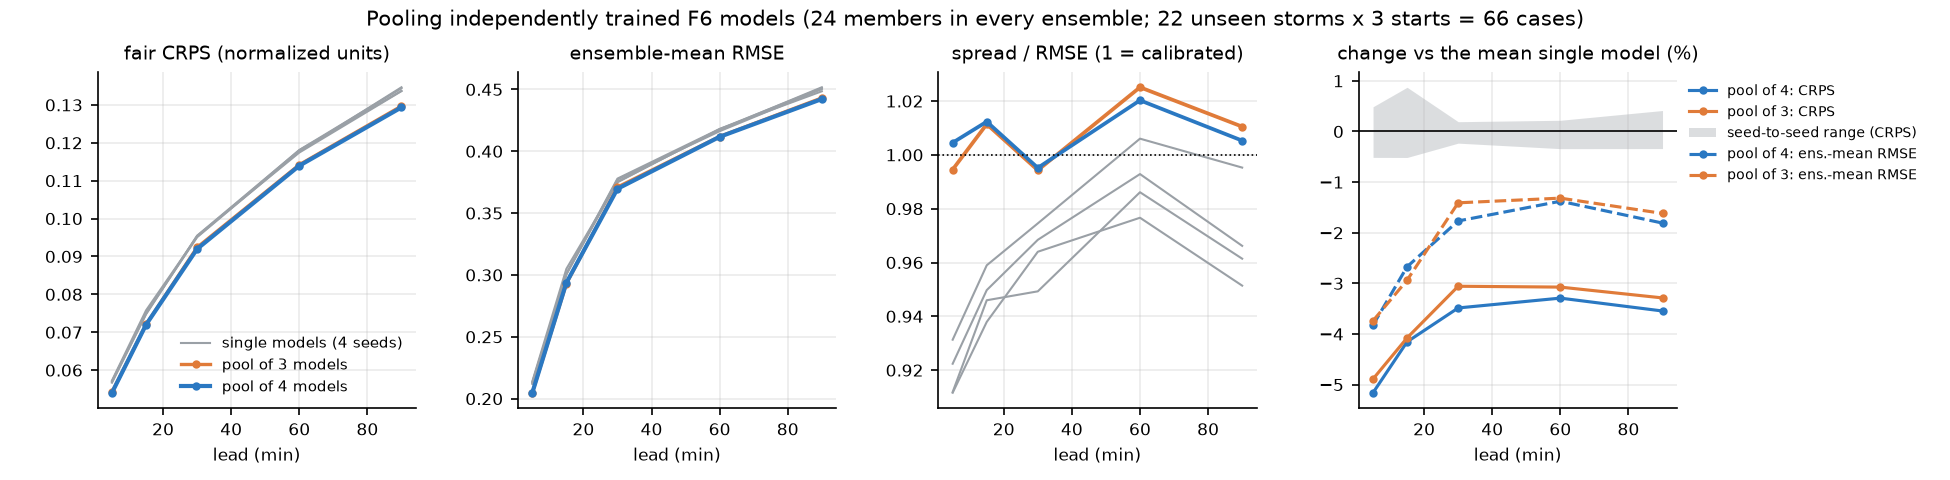
\includegraphics[width=\textwidth]{fig_pool_skill.png}
\caption{Single models (grey, four seeds) against pools of 3 and 4 models, all with 24 members. Right: change relative to the mean single model, with the seed-to-seed range of the CRPS shaded.}
\label{fig:skill}
\end{figure}

\begin{figure}[h]
\centering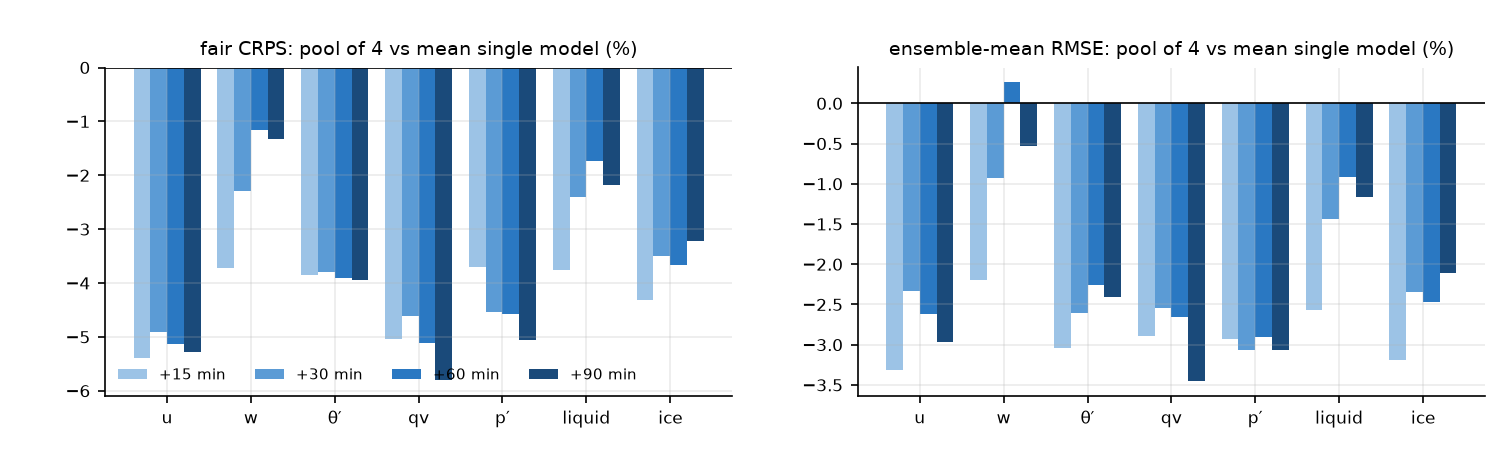
\includegraphics[width=\textwidth]{fig_pool_pervar.png}
\caption{Change of the pool of four relative to the mean single model, per variable and lead.}
\label{fig:pervar}
\end{figure}

\paragraph{The vote.} Figure~\ref{fig:voten} separates the effect of more members from the effect of more models. Each pool of $n$ models $\times$ 8 members is set against one model with the same $8n$ members.
\begin{itemize}
\item Both ensembles gain from more members. The pool gains more, and the gap is still growing at four models: $+0.009$, $+0.008$ and $+0.009$ in mean CSI over the 12 features at 15, 30 and 60\,min.
\item Against the 8-member vote of one model, the pool of four gains $+0.023$, $+0.022$ and $+0.026$.
\item The pool beats one model with 32 members for all 12 features at every lead (Fig.~\ref{fig:votefeat}).
\item The largest gains over the 8-member vote are in the features whose position is most uncertain. Downdraft CSI goes from 0.24 to 0.28 at 30\,min, the warm core from 0.52 to 0.55, and the mesolow from 0.42 to 0.44.
\item More members also bring the forecast area nearer the truth. The 8-member vote over-forecasts downdrafts at 2.1--2.3 times the true area; in the pool this falls to 1.5--1.6.
\end{itemize}

\begin{figure}[h]
\centering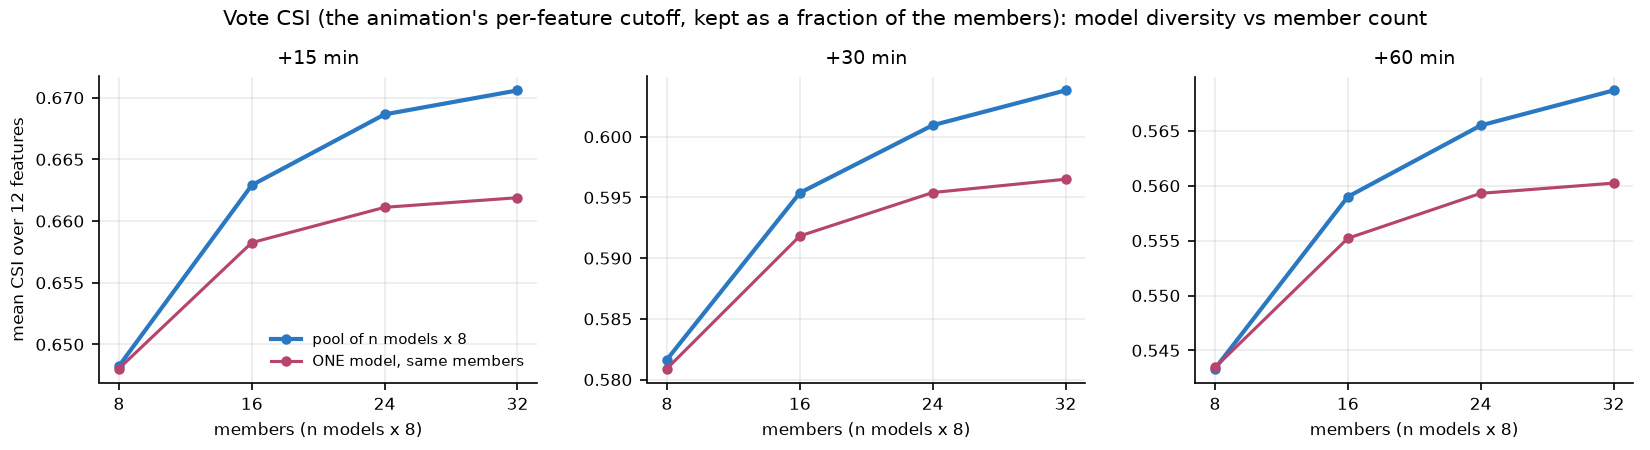
\includegraphics[width=\textwidth]{fig_pool_vote_n.png}
\caption{Mean CSI of the vote over 12 features: pools of $n$ independently trained models $\times$ 8 members (blue) against one model with the same number of members (red). 66 cases.}
\label{fig:voten}
\end{figure}

\begin{figure}[h]
\centering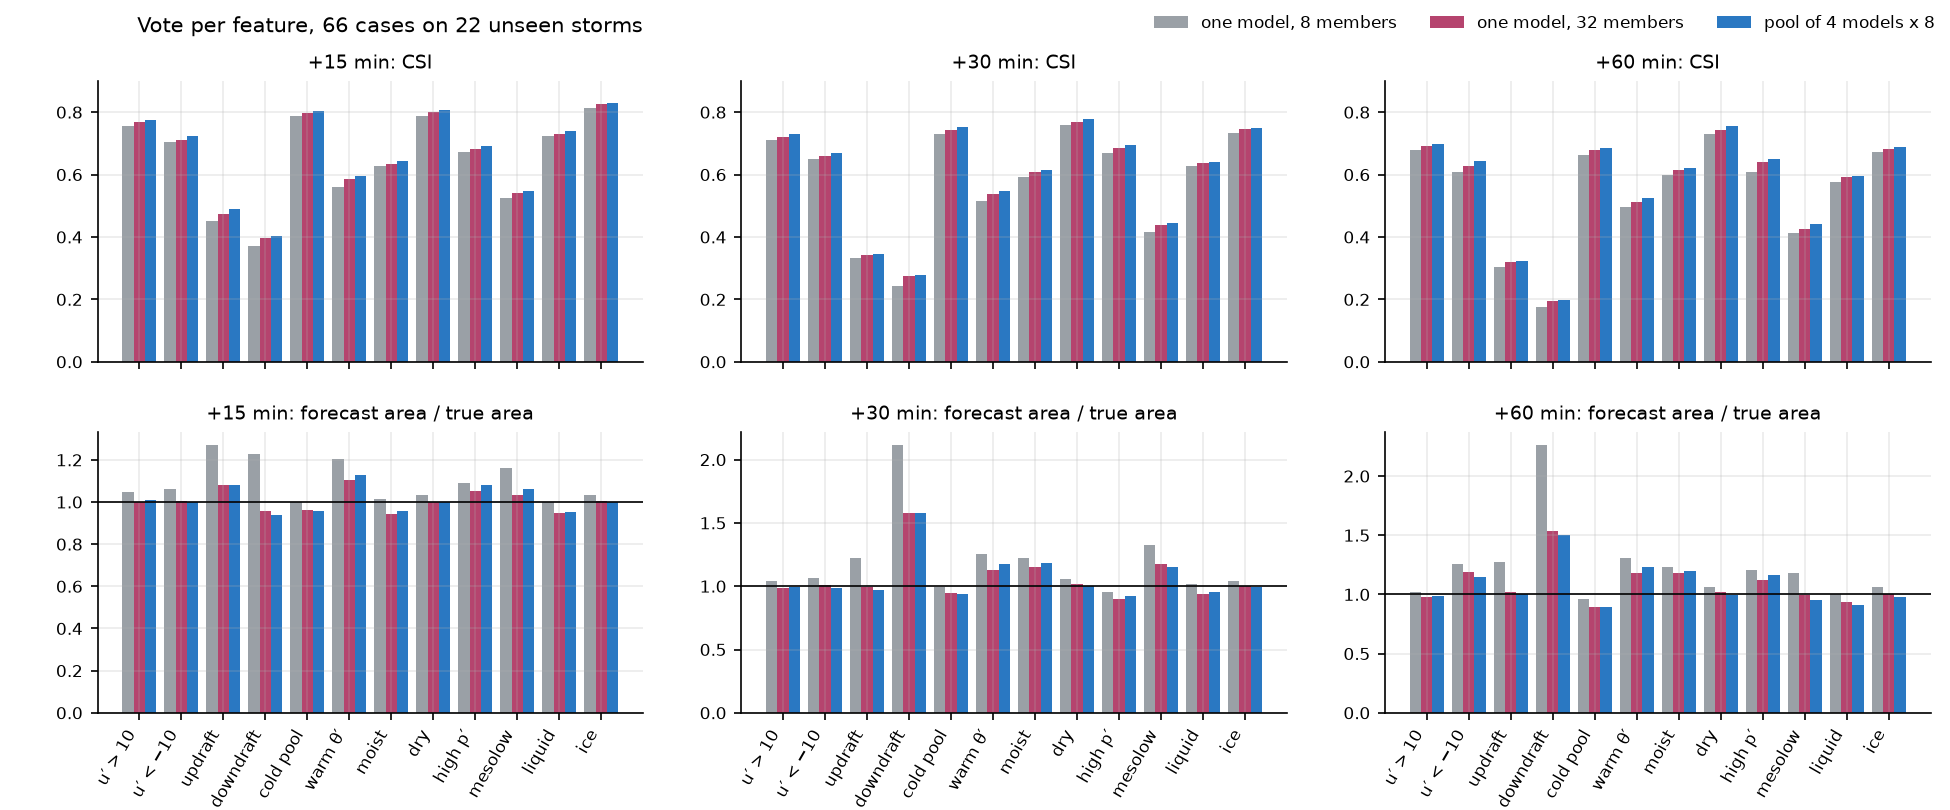
\includegraphics[width=\textwidth]{fig_pool_vote_feat.png}
\caption{Per-feature CSI (top) and forecast area / true area (bottom; 1 is unbiased): one model with 8 members, one model with 32, and the pool of four models $\times$ 8.}
\label{fig:votefeat}
\end{figure}

\IfFileExists{../fpe_report/figs_pool/fig_pool_vote_mem029_L30.png}{
\begin{figure}[h]
\centering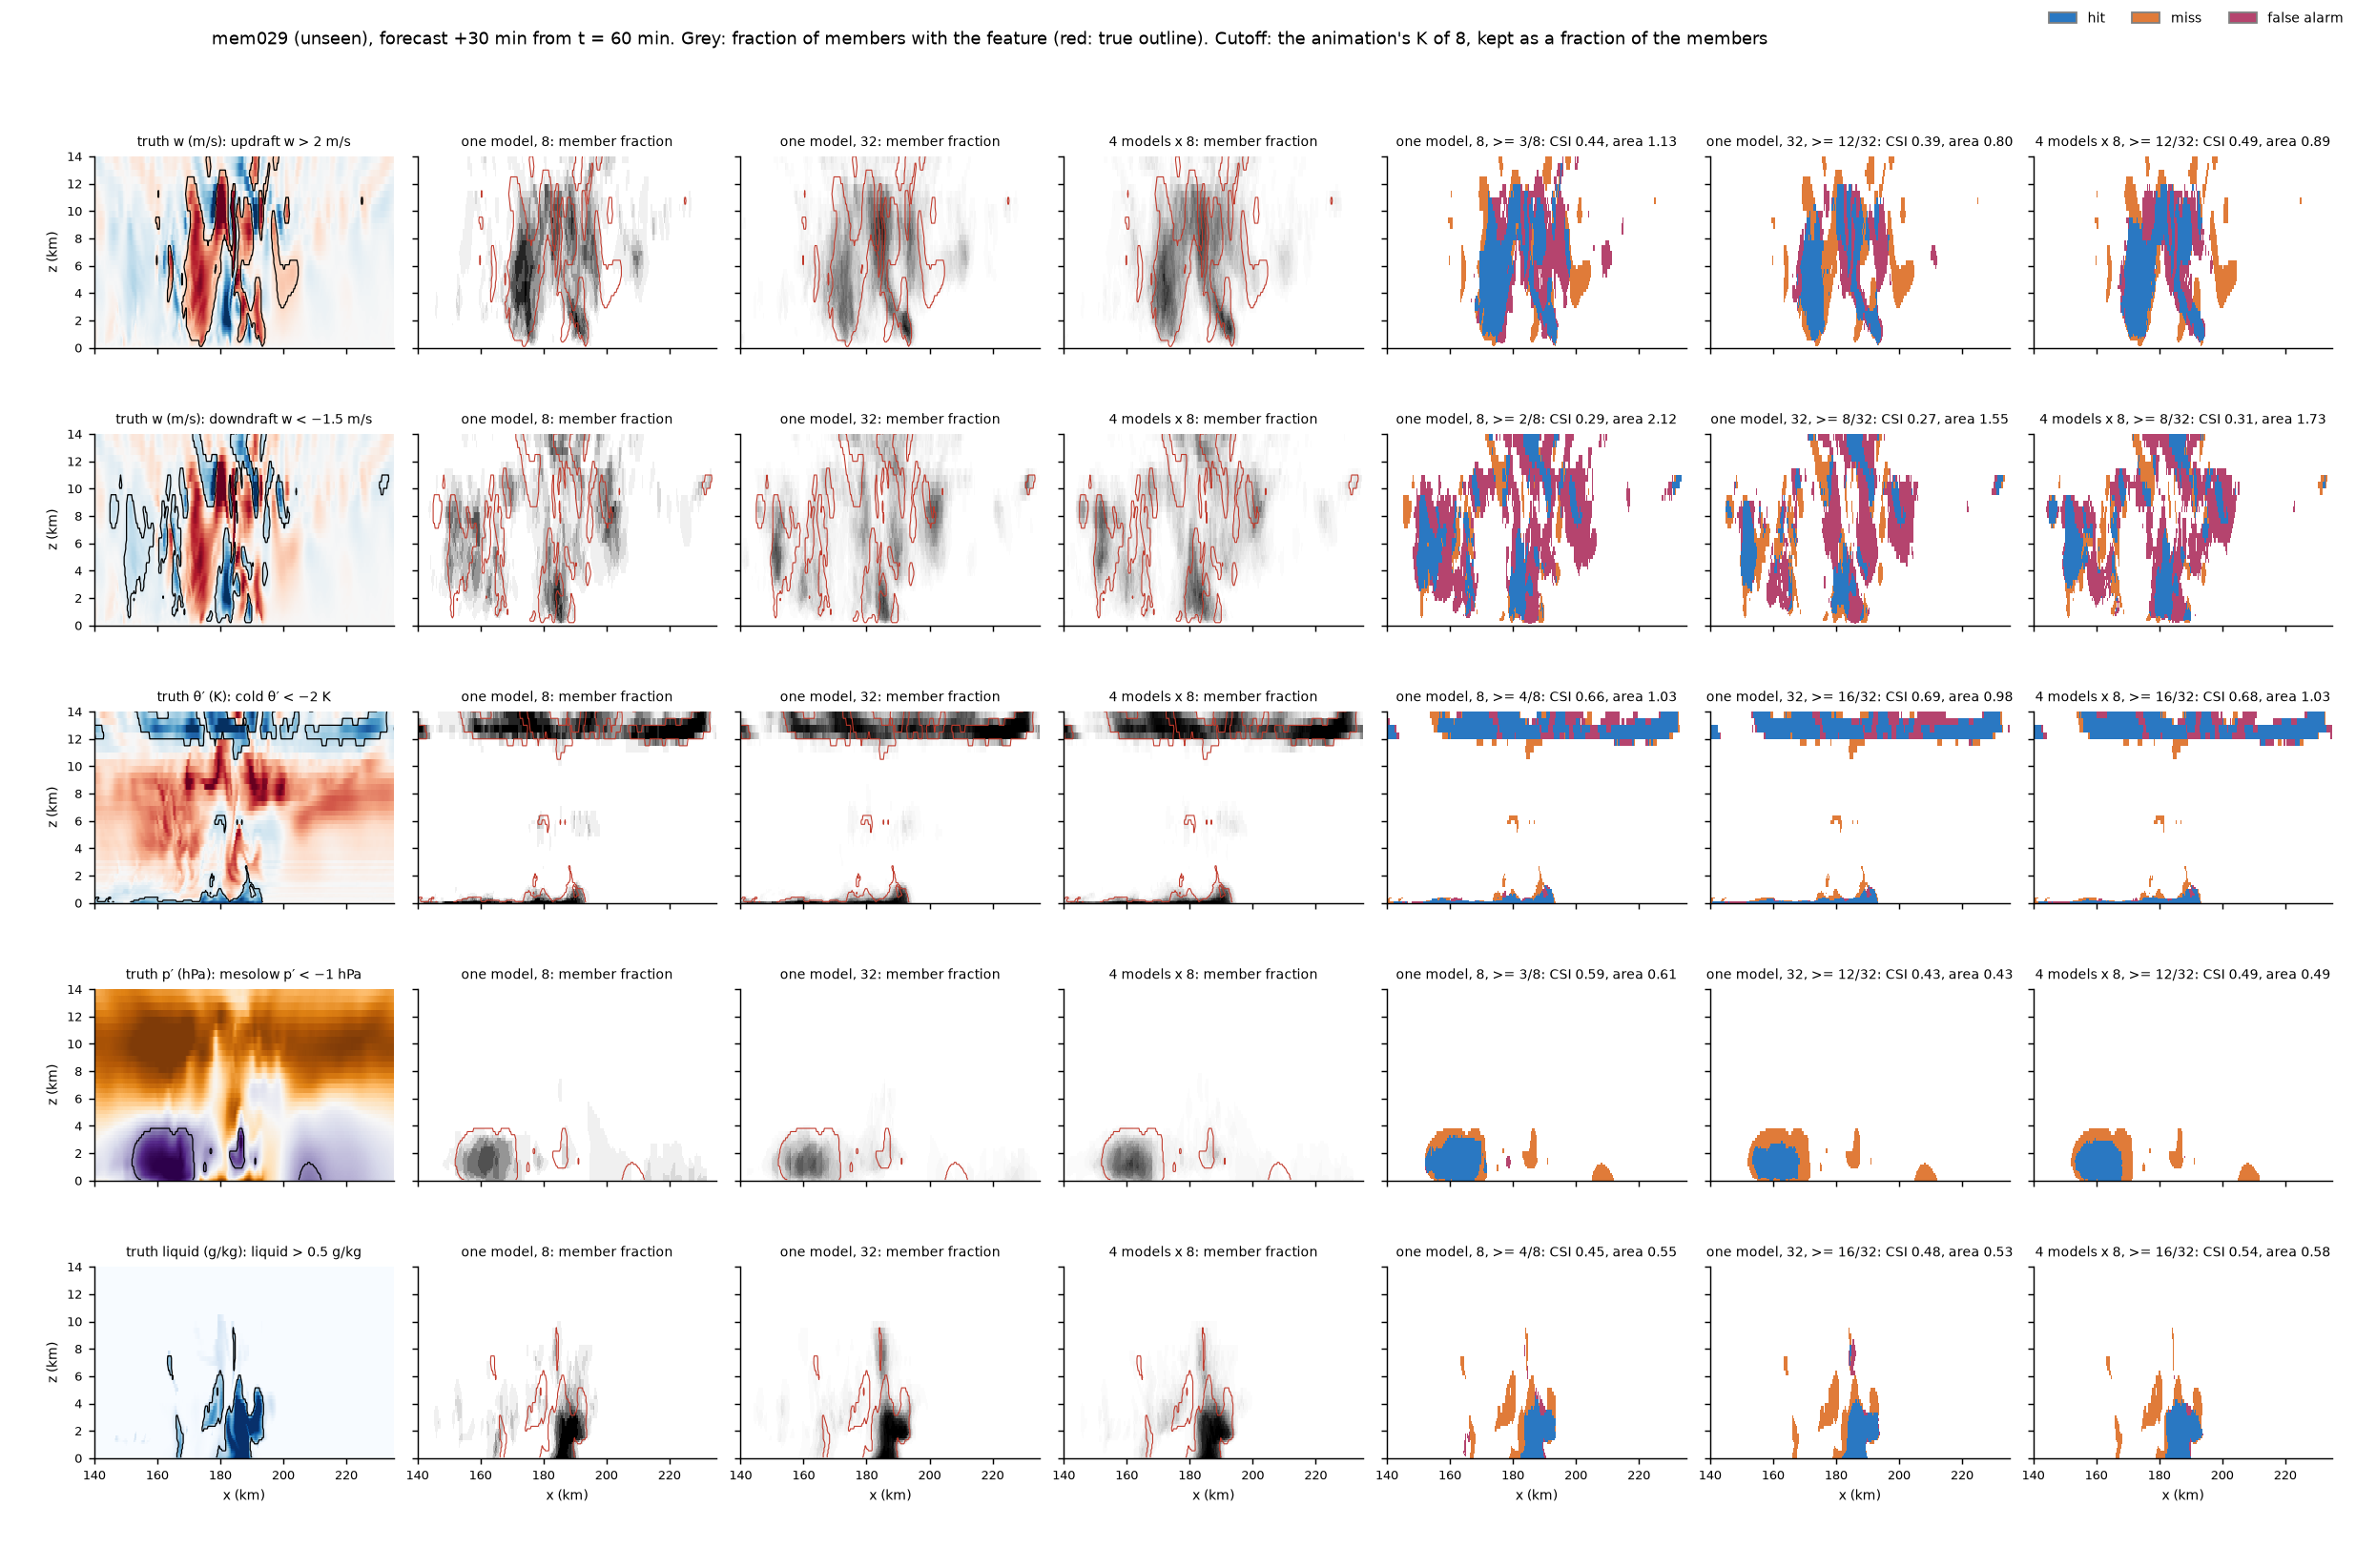
\includegraphics[width=\textwidth]{fig_pool_vote_mem029_L30.png}
\caption{One unseen storm, +30\,min. Left: the true field with the feature outlined. Middle: the fraction of members with the feature, for one model with 8 members, one model with 32, and the pool of 4 $\times$ 8. Right: the voted forecast as hits (blue), misses (orange) and false alarms (purple), with CSI and area ratio.}
\label{fig:map}
\end{figure}}{}

\FloatBarrier
\paragraph{Limits.}
\begin{itemize}
\item \emph{Small, fast features remain hard.} Updraft CSI is 0.35 at 30\,min and 0.32 at 60; downdraft CSI is 0.28 and 0.20. These features are forecast in the right region but rarely at the right grid point.
\item \emph{One environment.} All training storms share one sounding. On a first set of storms from new environments (varied CAPE from 800 to 4500\,J\,kg$^{-1}$, shear profiles and mid-level humidity; 6 storms, preliminary), CRPS at 30\,min is about twice its value on the test storms. Part of that comes from the stronger storms being harder to forecast.
\item \emph{Dying storms.} About a quarter of the new-environment storms decay, and the training set has none. Once a storm has died its fields are exactly zero, which the autoencoder cannot represent, and the forecasts fail.
\item \emph{Retraining under way.} The model is being retrained on 320 new-environment storms, including decaying ones.
\item \emph{Boundaries} come from the truth in these scores (see Setup).
\end{itemize}

\section{Could it be used with data assimilation?}

\paragraph{What makes it a good DA forecast model.}
\begin{itemize}
\item \emph{Calibrated spread.} An ensemble filter needs a prior spread that matches the forecast error. The pool provides this directly (spread/error 0.99--1.03 from 5 to 90\,min), without hand-set additive noise or heavy inflation.
\item \emph{Model error is represented.} Part of the pool's spread comes from disagreement between independently trained models, i.e.\ from model error. Ensemble DA usually has to add model error by hand (additive noise, multiplicative inflation, stochastic physics); here the forecast model supplies it.
\item \emph{Local latent field.} The latent state lives on 2\,km sites with a finite reach per step, so standard distance-based localization (e.g.\ a 5\,km LETKF radius on the site lattice) applies directly in latent space.
\item \emph{Cost.} A forecast hour of a 32-member ensemble takes a small fraction of a second on one GPU, so large ensembles and many cycles are cheap compared with running CM1.
\item \emph{The vote needs no change.} It acts on forecast members only, so forecasts launched from an analysis ensemble can be voted on exactly as above. Only the cutoffs need re-checking for that ensemble size.
\end{itemize}

\paragraph{What has to be solved.}
\begin{enumerate}
\item \emph{Several latent spaces.} Each model in the pool has its own encoder, so latent vectors from different models cannot share one covariance. There are three options:
  \begin{enumerate}
  \item update the decoded members in physical space, then re-encode each member with its own model's encoder. This is the simplest.
  \item run one latent LETKF per model, each with its own members. This keeps the latent update, but needs enough members per model for a usable covariance.
  \item train the pool's propagators on one shared, frozen autoencoder, so all members live in one latent space. This gives up the joint fine-tuning of stage C, and the cost of that has not been measured.
  \end{enumerate}
\item \emph{Inflation must be re-tuned.} Because the pool's spread is already calibrated, relaxation-to-prior or additive inflation tuned for a deterministic model would over-inflate it. Inflation should be tuned on the validation storms for this system.
\item \emph{Boundaries.} In a real cycle the halo cannot come from the truth. Holding it at the analysis value degrades long cycles and should be part of any test.
\item \emph{Robustness.} The model needs the retraining on new environments and decaying storms before DA results can be expected to hold beyond the training environment.
\end{enumerate}

\paragraph{Proposed test.} A twin experiment on the 22 test storms (3 observation-noise seeds each):
\begin{itemize}
\item \emph{Observations:} surface $\theta'$, composite reflectivity and radial velocity every 2\,km, assimilated every 5 minutes for 3\,h, with held boundaries.
\item \emph{Arms:} one model with 32 members; the pool of 4 $\times$ 8 updated in physical space; and the pool on a shared autoencoder updated in latent space. Inflation is tuned on the validation storms.
\item \emph{Scores:} cycled forecast error against no DA, gust-front position, spread/error and rank histograms at the observations, and the vote's CSI for forecasts launched from the analyses.
\end{itemize}
The prediction is that the pool's calibrated, model-error-aware spread will need little inflation and give lower cycled error than a single model with the same number of members. This has not yet been measured.

\end{document}
